% Large Language Models Section
\section{Large Language Models}

%------------------------------------------------
\subsection{What are Large Language Models}
%------------------------------------------------

%------------------------------------------------
\begin{frame}
\frametitle{Boom of Large Language Models}

\begin{columns}[c]

\column{.5\textwidth}
\begin{itemize}
\item \textbf{2017:} Transformer architecture introduced~\cite{vaswani2017attention}
\item \textbf{2018:} GPT-1, BERT~\cite{devlin2018bert}
\item \textbf{2019--2020:} GPT-2, GPT-3~\cite{brown2020language}
\item \textbf{2022:} ChatGPT ignites the AI boom~\cite{ouyang2022training}
\item \textbf{2023--2025:} GPT-4, Claude~\cite{anthropic2024claude}, Gemini~\cite{team2023gemini}, DeepSeek~\cite{deepseek2024deepseek}, Qwen~\cite{bai2023qwen}, and other multimodal models.
\end{itemize}

\column{.5\textwidth}
\centering
\includegraphics[width=\textwidth]{graphics/figures/llms/llms_history.png}
\captionof{figure}{Timeline of notable LLM releases from Transformer (2017) to recent multimodal systems.}

\end{columns}
\end{frame}
%------------------------------------------------

%------------------------------------------------
\begin{frame}
\frametitle{What are Large Language Models}

\begin{block}{Definition: Large Language Model}
A Large Language Model (LLM) is a parameterized conditional probability model, mapping any finite token sequence (context) to a probability distribution over
the next token in the vocabulary $\mathcal{V}$.  
The parameters $\theta$ are learned by maximizing log-likelihood over large-scale corpora~\cite{naveed2025comprehensive}.
\[
f_\theta:\mathcal{V}^* \rightarrow \Delta(\mathcal{V}),
\]
\end{block}

\vspace{0.4cm}

\textbf{Mathematical Notation}
\begin{itemize}
\item $\mathcal{V}$: token vocabulary (finite set of discrete symbols)
\item $\mathcal{V}^*$: the set of all finite-length sequences over $\mathcal{V}$  
(e.g., any prefix $w_{<t}$)
\item $\Delta(\mathcal{V})$: the probability simplex over $\mathcal{V}$  
\[
\Delta(\mathcal{V}) = 
\{ p:\mathcal{V}\to[0,1] \mid \sum_{v\in\mathcal{V}} p(v)=1 \}
\]
\item Induced joint distribution:
\[
P_\theta(w_{1:n})=\prod_{t=1}^n f_\theta(w_t \mid w_{<t})
\]
\end{itemize}

\end{frame}
%------------------------------------------------

%------------------------------------------------
\begin{frame}
\frametitle{Language Modeling}

\begin{block}{Language Modeling}
Language modeling estimates the joint distribution over a sequence
$w_{1:n}=(w_1,\ldots,w_n)$ by autoregressive factorization:
\[
P_\theta(w_{1:n})=\prod_{i=1}^{n}P_\theta(w_i\mid w_{<i}).
\]
\end{block}

\vspace{0.3cm}

\begin{block}{Training Objective}
Maximum likelihood (cross-entropy minimization):
\[
\mathcal{L}(\theta)
= -\sum_{i=1}^{n}\log P_\theta(w_i\mid w_{<i})
\quad\Longleftrightarrow\quad
\min_\theta \; \mathrm{CE}(P_{\text{data}},P_\theta).
\]
\end{block}

\vspace{0.2cm}

\end{frame}
%------------------------------------------------

%------------------------------------------------
\begin{frame}
\frametitle{Language Modeling Metrics}

\begin{itemize}
\item \textbf{Autoregressive generation:} 
The model predicts the next token given a prefix:
\[
w_{t+1} \sim P_\theta(\cdot \mid w_{\le t}),
\]

\item \textbf{Context window:}
The model conditions only on the most recent $L$ tokens:
\[
P_\theta(w_t \mid w_{<t}) \approx P_\theta(w_t \mid w_{t-L:t-1}).
\]

\item \textbf{Perplexity (PPL):}
For a sequence $w_{1:n}$, the average negative log-likelihood is
\[
\mathcal{L}(\theta)
= -\frac{1}{n}\sum_{t=1}^n \log P_\theta(w_t \mid w_{<t}).
\]
Perplexity is defined as:
\[
\mathrm{PPL}
= \exp\!\Big( \mathcal{L}(\theta) \Big)
= \exp\!\left( -\frac{1}{n}\sum_{t=1}^n \log P_\theta(w_t \mid w_{<t}) \right).
\]

\item \textbf{Interpretation:} Geometric mean of inverse probabilities. Lower is better.
\[
\mathrm{PPL} = \left( \prod_{t=1}^n \frac{1}{P_\theta(w_t \mid w_{<t})} \right)^{\!\frac{1}{n}}.
\]

\end{itemize}
\end{frame}
%------------------------------------------------

%------------------------------------------------
\subsection{Transformers}
%------------------------------------------------

%------------------------------------------------
\begin{frame}
\frametitle{Transformer Architecture}

\begin{block}{Core Innovation}
Transformers replace recurrence with self-attention, enabling parallel token interactions
and efficient modeling of long-range dependencies~\cite{vaswani2017attention}.
\end{block}

\vspace{0.3cm}

\textbf{Layer Structure (Encoder/Decoder block)}
Given hidden states $H\in\mathbb{R}^{n\times d}$:
\[
\tilde{H} = \mathrm{MHA}(H) + H,\qquad
H^{+} = \mathrm{FFN}(\tilde{H}) + \tilde{H}.
\]

\vspace{0.2cm}

\textbf{Key Components}
\begin{itemize}
\item \textbf{Self-attention} using learned projections $(W_Q, W_K, W_V)$.
\item \textbf{Multi-head attention} to attend in multiple subspaces.
\item \textbf{Positional encoding} to inject sequence order.
\item \textbf{Position-wise feed-forward network} for nonlinearity and mixing.
\item \textbf{Residual connections + LayerNorm} for stable optimization.
\end{itemize}
\end{frame}

%------------------------------------------------

\begin{frame}
\frametitle{Self-Attention Mechanism}

\textbf{Construction:}
For hidden states $H \in \mathbb{R}^{n \times d}$,
\[
Q = HW_Q,\quad K = HW_K,\quad V = HW_V,
\]
with projection matrices $W_Q, W_K, W_V \in \mathbb{R}^{d \times d}$.
In multi-head attention, $Q,K,V$ are reshaped into $h$ heads.

\vspace{0.3cm}

\begin{block}{Scaled Dot-Product Attention~\cite{vaswani2017attention}}
\[
\mathrm{Attention}(Q,K,V)
= \mathrm{softmax}\!\left(\frac{QK^\top}{\sqrt{d_k}}\right)V.
\]
\end{block}

\vspace{0.3cm}

\textbf{Multi-Head Attention (MHA):}
\[
\mathrm{MHA}(H)=\mathrm{Concat}(\mathrm{head}_1,\ldots,\mathrm{head}_H)W_O.
\]

\end{frame}
%------------------------------------------------

%------------------------------------------------
\begin{frame}
\frametitle{Decoding Strategies in Large Language Models}

\begin{columns}[T]

\column{0.48\textwidth}

\textbf{Greedy Decoding}
\[
w_{t+1} = \arg\max_{w} P_\theta(w \mid w_{\le t})
\]
Deterministic but often repetitive.

\vspace{0.3cm}

\textbf{Temperature Sampling}
Rescales logits before softmax:
\[
P_T(w_i) = \frac{\exp(z_i / T)}{\sum_j \exp(z_j / T)}
\]
$T < 1$: sharper; $T > 1$: more random.

\vspace{0.3cm}

\textbf{Top-$k$ Sampling}
Sample only from the $k$ most probable tokens.

\column{0.48\textwidth}

\textbf{Top-$p$ (Nucleus) Sampling}
Use smallest set $V_p$ covering probability mass $p$~\cite{holtzman2019curious}:
\[
\sum_{i \in V_p} P(w_i) \ge p.
\]
Adaptive truncation prevents tail degeneration.

\vspace{0.3cm}

\textbf{Beam Search}
Maintains $B$ candidate sequences:
\[
\max_{w_{1:T}} 
\sum_{t=1}^{T} 
\log P_\theta(w_t \mid w_{<t})
\]
Effective for translation; less suitable for open-ended chat.

\end{columns}

\end{frame}
%------------------------------------------------

%------------------------------------------------
\begin{frame}
\frametitle{Temperature: Effect on Softmax Distribution}

\begin{figure}[t]
    \centering
    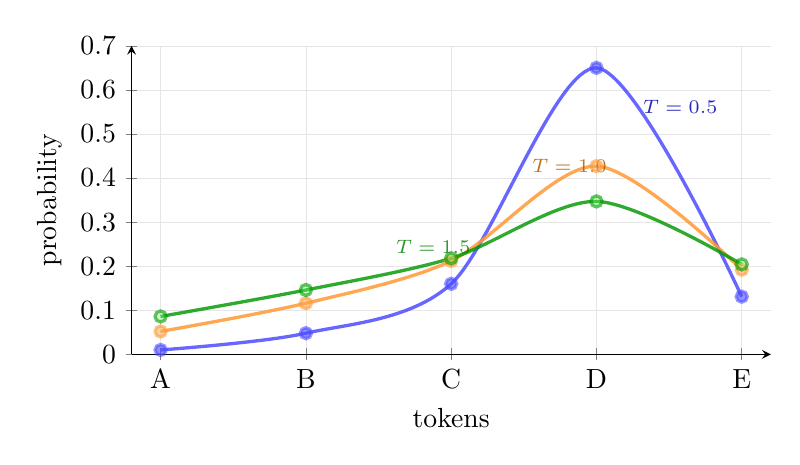
\begin{tikzpicture}
        \begin{axis}[
            width=0.8\linewidth,
            height=5.5cm,
            axis lines=left,
            xmin=-0.2, xmax=4.2,
            ymin=0, ymax=0.7,
            xtick={0,1,2,3,4},
            xticklabels={A,B,C,D,E},
            ytick={0,0.1,0.2,0.3,0.4,0.5,0.6,0.7},
            xlabel={tokens},
            ylabel={probability},
            grid=both,
            grid style={line width=0.2pt, draw=gray!20},
            legend style={draw=none, fill=none, font=\small},
            legend pos=north east,
            clip=false
        ]
            % Sharper: T=0.5
            \addplot+[smooth, very thick, draw=blue!70, opacity=0.85, mark=*,
                    mark options={fill=blue!70,fill opacity=0.6,draw opacity=0.6}]
                coordinates {(0,0.01) (1,0.048) (2,0.16) (3,0.65) (4,0.131)}
                node[pos=0.8, above right, font=\scriptsize, text=blue!70!black]{$T=0.5$};
            % Base: T=1.0
            \addplot+[smooth, very thick, draw=orange!80!white, opacity=0.85, mark=*,
                    mark options={fill=orange!70,fill opacity=0.45,draw opacity=0.6}]
                coordinates {(0,0.052) (1,0.116) (2,0.212) (3,0.427) (4,0.192)}
                node[pos=0.7, above, font=\scriptsize, text=orange!70!black]{$T=1.0$};
            % Flatter: T=1.5
            \addplot+[smooth, very thick, draw=green!60!black, opacity=0.82, mark=*,
                    mark options={fill=green!55,fill opacity=0.35,draw opacity=0.6}]
                coordinates {(0,0.086) (1,0.146) (2,0.218) (3,0.347) (4,0.204)}
                node[pos=0.55, left, font=\scriptsize, text=green!50!black]{$T=1.5$};
        \end{axis}
    \end{tikzpicture}
\end{figure}

\vspace{0.15cm}
\captionof{figure}{Temperature scaling reshapes the same logits.}

\end{frame}

%------------------------------------------------
\begin{frame}
\frametitle{Beam Search (Beam Width $B=2$)}

\begin{figure}[t]
\centering
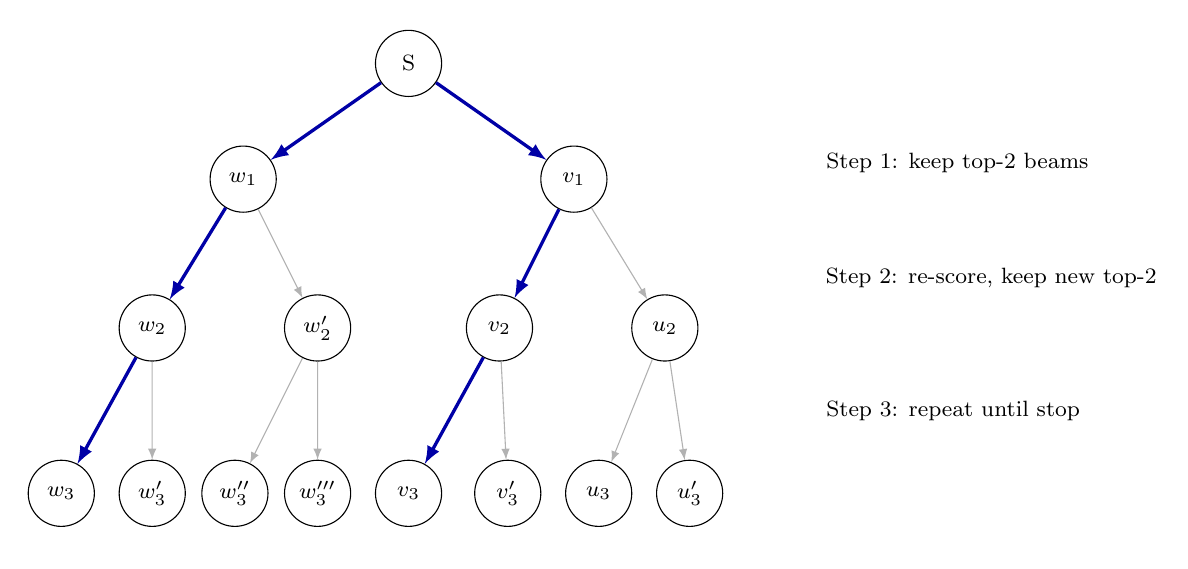
\begin{tikzpicture}[
    scale=1.05,
    yshift=-3mm,
    >=latex,
    every node/.style={circle,draw,minimum size=8.4mm,inner sep=1.2pt,font=\footnotesize},
    beam/.style={very thick,blue!65!black},
    pruned/.style={draw=gray!60,text=gray!80},
    every path/.style={-latex}
]
% Nodes laid out top-to-bottom (t = 0,1,2,3)
\node (s)   at (0,-0.6)        {S};
\node (a1)  at (-2.0,-2.0)  {$w_1$};
\node (c1)  at ( 2.0,-2.0)  {$v_1$};
\node (a2)  at (-3.1,-3.8)  {$w_2$};
\node (b2)  at (-1.1,-3.8)  {$w'_2$};
\node (c2)  at ( 1.1,-3.8)  {$v_2$};
\node (d2)  at ( 3.1,-3.8)  {$u_2$};
\node (a3)   at (-4.2,-5.8) {$w_3$};
\node (a3b)  at (-3.1,-5.8) {$w'_3$};
\node (b3)   at (-2.1,-5.8) {$w''_3$};
\node (b3b)  at (-1.1,-5.8) {$w'''_3$};
\node (c3)   at ( 0.0,-5.8) {$v_3$};
\node (c3b)  at ( 1.2,-5.8) {$v'_3$};
\node (d3)   at ( 2.3,-5.8) {$u_3$};
\node (d3b)  at ( 3.4,-5.8) {$u'_3$};

% Step 1: expand root, keep top-2
\onslide<1->{\draw[beam] (s) -- (a1);}
\onslide<1->{\draw[beam] (s) -- (c1);}
\onslide<1->{\node[anchor=west,draw=none] at (5.0,-1.8) {\footnotesize Step 1: keep top-2 beams};}
% Step 2: expand kept beams
\onslide<2->{\draw[beam] (a1) -- (a2);}
\onslide<2->{\draw[pruned] (a1) -- (b2);}
\onslide<2->{\draw[beam] (c1) -- (c2);}
\onslide<2->{\draw[pruned] (c1) -- (d2);}
\onslide<2->{\node[anchor=west,draw=none] at (5.0,-3.2) {\footnotesize Step 2: re-score, keep new top-2};}
% Step 3: expand again
\onslide<3->{\draw[beam] (a2) -- (a3);}
\onslide<3->{\draw[pruned] (a2) -- (a3b);}
\onslide<3->{\draw[pruned] (b2) -- (b3);}
\onslide<3->{\draw[pruned] (b2) -- (b3b);}
\onslide<3->{\draw[beam] (c2) -- (c3);}
\onslide<3->{\draw[pruned] (c2) -- (c3b);}
\onslide<3->{\draw[pruned] (d2) -- (d3);}
\onslide<3->{\draw[pruned] (d2) -- (d3b);}
\onslide<3->{\node[anchor=west,draw=none] at (5.0,-4.8) {\footnotesize Step 3: repeat until stop};}

\end{tikzpicture}
\caption{\hspace{0.6em}Beam width $B=2$: expand all candidates each step, keep the two highest-scoring prefixes (blue).}
\end{figure}

\end{frame}
%------------------------------------------------

%------------------------------------------------
\subsection{Pre-Training and Fine-Tuning}
%------------------------------------------------
\begin{frame}
\frametitle{Training Paradigm Evolution}

\textbf{From Pretraining to Alignment}
\begin{itemize}
    \item \textbf{Pretraining:} large-scale next-token prediction~\cite{brown2020language}.
    \[
    \min_\theta -\sum_{t}\log P_\theta(w_t \mid w_{<t})
    \]
    Foundation model learns general linguistic and world knowledge.

    \item \textbf{Fine-tuning (general concept):}
    adapt pretrained parameters $\theta_0$ to a new distribution:
    \[
    \theta^{*} = \arg\max_\theta 
    \sum_{(x,y)\in \mathcal{D}_{ft}}
    \log P_\theta(y \mid x)
    \]
    Includes SFT, RLHF, RLAIF, DPO~\cite{rafailov2023direct}, etc.
\end{itemize}

\vspace{0.3cm}
Modern alignment pipeline:
\[
\text{Pretraining} 
~\rightarrow~ 
\text{SFT}
~\rightarrow~ 
\text{Preference Optimization (RLHF / RLAIF)}
\]

\end{frame}

%------------------------------------------------
\begin{frame}
\frametitle{Modern Alignment Techniques} 
\vspace{0.3cm}

\textbf{Supervised Fine-Tuning (SFT)}
\begin{itemize}
    \item Dataset of instruction–response pairs $\mathcal{D}_{SFT}=\{(x_i, y_i)\}$.
    \item Optimize cross-entropy (teacher forcing)~\cite{ouyang2022training}.
    \item Teaches format, compliance, basic helpfulness.
\end{itemize}

\vspace{0.2cm}
\textbf{Reinforcement Learning from Human Feedback (RLHF)}
\begin{itemize}
    \item \textbf{Reward Model (RM)} trained on preference pairs~\cite{christiano2017deep}.
    \item \textbf{PPO optimization} with KL constraint:
    \[
    \max_{\theta}
    \mathbb{E}[\,r_\phi(x,y)\,]
    - \beta \,\mathrm{KL}(\pi_\theta \| \pi_{SFT})
    \]
    \item Improves helpfulness, harmlessness, and alignment.
\end{itemize}

\end{frame}

%------------------------------------------------
\begin{frame}
\frametitle{RLAIF and Scalable Oversight}

\textbf{Reinforcement Learning from AI Feedback (RLAIF)}
\begin{itemize}
    \item Replace human preference labels with a strong AI judge.
    \item Construct AI preference pairs $(x, y^{+}, y^{-})_{\text{AI}}$~\cite{bai2022constitutional}.
    \item Enables scalable, cheaper, principle-based alignment (Constitutional AI).
\end{itemize}

\vspace{0.3cm}
\textbf{Training Paradigm Summary}
\begin{itemize}
    \item \textbf{SFT}: learns to follow instructions.
    \item \textbf{RLHF}: aligns to human preferences.
    \item \textbf{RLAIF}: aligns via AI-based preference judgments.
\end{itemize}

\vspace{0.2cm}
\[
\text{SFT: “can talk”} 
\quad\Rightarrow\quad
\text{RLHF/RLAIF: “talks well”}
\]

\end{frame}


%------------------------------------------------
\subsection{Mainstream LLMs}
%------------------------------------------------

\begin{frame}
\frametitle{Major LLM Families}

\begin{columns}[T]

\column{.5\textwidth}
\textbf{Decoder-Only Models (Autoregressive)}
\begin{itemize}
\item GPT Series (OpenAI)~\cite{brown2020language}
\item LLaMA (Meta)~\cite{touvron2023llama}
\item Qwen (Alibaba)~\cite{bai2023qwen}
\item Mistral / Mixtral (MoE)~\cite{jiang2023mistral}
\item DeepSeek~\cite{deepseek2024deepseek}
\end{itemize}

\vspace{0.3cm}

\textbf{Encoder-Only Models (Bidirectional)}
\begin{itemize}
\item BERT (Google)~\cite{devlin2018bert}
\item RoBERTa, ALBERT
\item Focused on understanding tasks
\end{itemize}

\column{.5\textwidth}
\textbf{Encoder--Decoder Models (Seq2Seq)}
\begin{itemize}
\item T5 / FLAN-T5~\cite{raffel2020exploring}
\item Strong for translation, summarization
\end{itemize}

\vspace{0.3cm}

\textbf{Multimodal Models}
\begin{itemize}
\item GPT-4 / GPT-4o (OpenAI)
\item Gemini (Google)~\cite{team2023gemini}
\item Claude 3 (Anthropic)~\cite{anthropic2024claude}
\end{itemize}

\end{columns}
\end{frame}

%------------------------------------------------

\begin{frame}
\frametitle{Notable Architectures and Innovations}

\textbf{Open-Source Ecosystem:}
\begin{itemize}
\item \textbf{LLaMA}: flexible scales, strong baseline for fine-tuning.
\item \textbf{Mistral/Mixtral}: efficient attention, MoE routing~\cite{jiang2023mistral}.
\item \textbf{DeepSeek}: optimized training pipeline and inference efficiency~\cite{deepseek2024deepseek}.
\end{itemize}

\vspace{0.3cm}

\textbf{Key Innovations:}
\begin{itemize}
\item \textbf{MoE (Mixture of Experts):} Activates only a subset of parameters per token (Mistral, DeepSeek).
\item \textbf{Long Context:} Handling 1M+ tokens (Gemini, Claude).
\item \textbf{Attention Efficiency:} FlashAttention, RoPE, ALiBi.
\end{itemize}

\end{frame}

%------------------------------------------------
\subsection{Capabilities and Limitations}
%------------------------------------------------
\begin{frame}
\frametitle{Capabilities of Large Language Models}

\textbf{Core Strengths of LLMs~\cite{naveed2025comprehensive}}
\begin{itemize}
    \item \textbf{Language Generation:} Produce coherent, context-aware text.
    \item \textbf{Semantic Understanding:} Encode rich contextual representations.
    \item \textbf{In-Context Learning:} Adapt to new tasks from examples without updates~\cite{brown2020language}.
    \item \textbf{Reasoning Heuristics:} Chain-of-thought, code synthesis.
    \item \textbf{Multimodal Integration:} Align text, image, audio.
    \item \textbf{Knowledge Compression:} Store world knowledge in parameters.
\end{itemize}

\vspace{0.25cm}
LLMs are powerful \textit{latent knowledge engines}.
\end{frame}


%------------------------------------------------
\begin{frame}
\frametitle{Limitations \& Motivation for AI Agents}

\textbf{Fundamental Limitations~\cite{sapkota2025ai}}
\begin{itemize}
    \item \textbf{Lack of Groundedness:} No direct access to real-time information.
    \item \textbf{No Persistent Memory:} Context is bounded.
    \item \textbf{Unreliable Reasoning:} Hallucinations.
    \item \textbf{Static Knowledge:} Knowledge is “frozen” at training time.
    \item \textbf{Weak Action Capabilities:} Cannot execute actions reliably.
\end{itemize}

\vspace{0.3cm}

\textbf{Why AI Agents?}
\begin{itemize}
    \item Integrate LLMs with \textbf{tools}, \textbf{memory}, \textbf{environment}~\cite{weng2023prompt}.
    \item Enable planning, real-world actions, continual information gathering.
    \item Transform LLMs from passive text generators to \textbf{autonomous problem-solvers}.
\end{itemize}

\end{frame}